\documentclass[10pt,a4paper]{amsart}
% \documentclass[10pt,a4paper]{article}
\usepackage[utf8x]{inputenc}
\usepackage{ucs}
\usepackage[brazil]{babel}
\usepackage[T1]{fontenc}
\usepackage{amsmath}
\usepackage{amsfonts}
\usepackage{amssymb}
\usepackage{indentfirst}
%to bind figures in respective sections
\usepackage[section]{placeins}
%to number figures considering the section
\usepackage{chngcntr}
\counterwithin{figure}{section}

%for pseudocode
% \usepackage[]{algorithm2e}
\usepackage{algorithm}
\usepackage[noend]{algpseudocode}
\makeatletter
\def\BState{\State\hskip-\ALG@thistlm}
\makeatother
\floatname{algorithm}{Algoritmo}
\renewcommand{\algorithmicrequire}{\textbf{Entrada:}}
\renewcommand{\algorithmicensure}{\textbf{Saída:}}
\renewcommand{\algorithmicwhile}{\textbf{Enquanto}}
\renewcommand{\algorithmicdo}{\textbf{faça}}
\renewcommand{\algorithmicfor}{\textbf{Para}}
\renewcommand{\algorithmicif}{\textbf{Se}}
\renewcommand{\algorithmicthen}{\textbf{então}}

% for pretty-printed source code
\usepackage{listings}
% environment for C code
\lstnewenvironment{code}
 {\lstset{ %
     extendedchars=true,
     stringstyle=\ttfamily \scriptsize, %
     showstringspaces=false, aboveskip={1.\baselineskip}, %
     identifierstyle=\ttfamily \scriptsize \bf, %
     language=C,           %
     basicstyle=\ttfamily \small,  %\footnotesize
     numberstyle=\footnotesize, %
     % keywordstyle=\bf,       % keyword style
     tabsize=1,                 % sets default tabsize to 2 spaces
     captionpos=t,              % sets the caption-position to bottom
     breaklines=true,           % sets automatic line breaking
     breakatwhitespace=false,   % sets if automatic breaks should only happen at whitespace
     %backgroundcolor=\color{black!10},
   }
} {}

\author{Jo\~ao S. Brito Jr.\\NUSP: 5889672}
\title{Modelos Probabilísticos Baseados em Grafos: \\Aprendizado e Classificação}
\date{\today}
\usepackage{graphicx}
\graphicspath{ {images/} }

\begin{document}

% \begin{abstract}
%   % Resumo
%   Este documento descreve...
% \end{abstract}

\maketitle

\section{Introdução}

\section{Background}
%   conceitos, notações
\section{Descrição dos Algoritmos}
%   aqui pode incluir pseudocódigo e descrição
\subsection{Iteração de Valor}
\subsection{Iteração de Valor Topológica}
\subsection{Instruções de Execução}
\subsection{Principais dificuldades encontradas na implementação}

%FOCAR NESTA SEÇÃO DESTA VEZ !!!!!!!!!!!!!!!!!!!!!!!!!!!!!!!!!!!!!
\section{Experimentos e Discussão}
%FOCAR NESTA SEÇÃO DESTA VEZ !!!!!!!!!!!!!!!!!!!!!!!!!!!!!!!!!!!!!

% configuração dos experimentos: computador, parâmetros utilizados
% analisar resultados:
% (acurácia, eficiência computacional, facilidade de implementação etc.)

Todos os experimentos foram efetuados em uma máquina com processador Intel Core 2 Duo 2.10GHz com 4GB de memória.

% As figuras abaixo mostram os resultados obtidos:
% Fig. ~\ref{fig:mid_layer_2_10}
% \begin{figure}[ht]
%   \centering
%   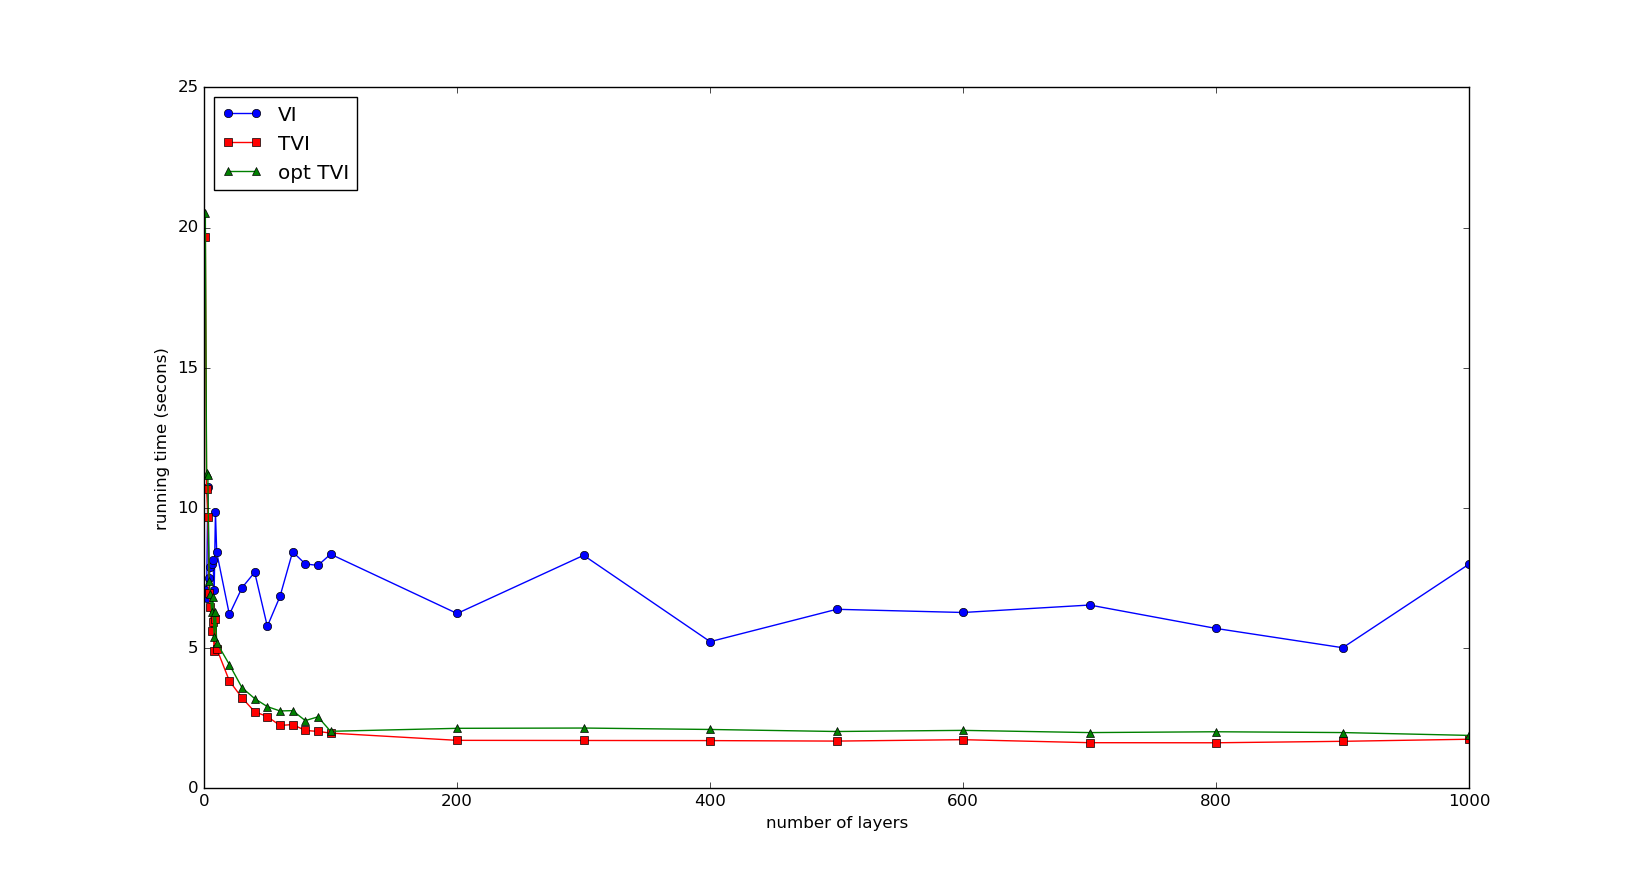
\includegraphics[width=\textwidth]{mid_layer_2_10}
%   \caption{Tempo em função do número de camadas. Problemas SSP gerados artificialmente com 5000 estados, 10 ações por estado, máximo de 10 sucessores por ação. Custo aleatório entre 2 e 10.}
%   \label{fig:mid_layer_2_10}
% \end{figure}

\section{Conclusão}

% \begin{thebibliography}{9}
% \bibitem{dai11}
%   Dai, P., Weld, D. S., Goldsmith, J. (2011). Topological value iteration algorithms. Journal of Artificial Intelligence Research, 181-209.
% \end{thebibliography}

\end{document}
